\documentclass[11pt,a4paper]{article}

% ---------- PACKAGES ----------
\usepackage{amsmath, amssymb, amsthm}
\usepackage{graphicx}
\usepackage{geometry}
\usepackage{hyperref}
\usepackage{float}
\usepackage{caption}
\usepackage{booktabs}
\usepackage{siunitx}
\usepackage{fancyhdr}

\geometry{margin=1in}
\hypersetup{
    colorlinks=true,
    linkcolor=blue,
    urlcolor=blue,
    citecolor=blue
}

\pagestyle{fancy}
\fancyhead[L]{Numerical Behavior of the Zeta Function}
\fancyhead[R]{J. Orellana}

% ---------- TITLE ----------
\title{\textbf{Numerical Behavior of the Riemann Zeta Function using Real-to-Complex Conversion}}
\author{Jacob Orellana Real\\
\small Independent Researcher\\
\small \texttt{jacoboreore@gmail.com}}
\date{\today}

\begin{document}

\maketitle

\begin{abstract}
The Riemann Zeta function $\zeta(s)$ lies at the heart of analytic number theory, encoding the distribution of primes through its non-trivial zeros. 
This paper introduces a direct computational framework for evaluating $Z(t) = e^{i\theta(t)}\zeta(\frac{1}{2}+it)$ at large imaginary parts $t$, employing a real-to-complex number conversion and a novel \emph{valley scanner} algorithm. 
The method efficiently identifies zeros by tracking minima of $|Z(t)|$, achieving stability and precision up to $t \approx 10^{20}$ with moderate computational cost, using AWS EC2 computation.
Results are compared against known Andrew Odlyzko zero datasets, validating the method’s accuracy while simplifying the high-$t$ evaluation pipeline.
\end{abstract}

\newpage
\tableofcontents

\newpage
\section{Introduction}
\label{sec:intro}
% --- Context & Motivation ---
The Riemann Hypothesis remains one of the most profound unsolved problems in mathematics. 
Its verification, even to limited numerical ranges, demands accurate computation of the function $\zeta(s)$ along the critical line $\Re(s) = \tfrac{1}{2}$.
Traditional methods rely on the Riemann–Siegel formula and Gram point interpolation, which become computationally intensive as $t$ grows large.
This paper presents a complementary approach based on direct numerical conversion of real inputs to complex domains, combined with a \emph{valley scanning} technique that efficiently isolates zeros without requiring Gram alignment.

\section{Mathematical Background}
\label{sec:background}

\subsection{The Riemann Zeta Function}

The Riemann zeta function is one of the most studied objects in mathematics, intimately connected to the distribution of prime numbers.  
For complex arguments \( s = \sigma + it \) with real part \( \sigma > 1 \), it is defined by the absolutely convergent series:
\[
\zeta(s) = \sum_{n=1}^{\infty} \frac{1}{n^s}.
\]

Through analytic continuation, this definition extends to all complex \( s \neq 1 \), and the function satisfies a deep symmetry captured by the \textbf{functional equation}:
\[
\zeta(s) = 2^s \pi^{s-1} \sin\!\left(\frac{\pi s}{2}\right)
\Gamma(1-s)\, \zeta(1-s),
\]
where \( \Gamma(s) \) is the Gamma function.  
This reflection property allows values of \( \zeta(s) \) on the right half-plane (\( \Re(s) > 1 \)) to determine those on the left.

The nontrivial zeros of \( \zeta(s) \) are the complex numbers \( s = \sigma + it \) that satisfy \( 0 < \sigma < 1 \) and \( \zeta(s) = 0 \).  
The celebrated \textbf{Riemann Hypothesis} conjectures that all such zeros lie on the critical line:
\[
\Re(s) = \tfrac{1}{2}.
\]

\subsection{Relation to Prime Numbers}

The zeta function encodes the structure of the primes through the \textbf{Euler product}:
\[
\zeta(s) = \prod_{p\,\text{prime}} \frac{1}{1 - p^{-s}}, \quad \Re(s) > 1,
\]
demonstrating that the analytic behavior of \( \zeta(s) \) reflects the multiplicative structure of the integers.  
In particular, zeros of \( \zeta(s) \) govern the distribution of primes via the explicit formula relating the prime-counting function \(\pi(x)\) and the zeros of \( \zeta(s) \):
\[
\pi(x) \sim \operatorname{Li}(x) - \sum_{\rho} \operatorname{Li}(x^{\rho}) + \text{(small correction terms)},
\]
where the sum runs over nontrivial zeros \( \rho = \tfrac{1}{2} + i t_\rho \).

\subsection{The Hardy Function \(Z(t)\)}

To facilitate numerical computation and visualization on the critical line, it is convenient to introduce the \textbf{Hardy function}:
\[
Z(t) = e^{i\theta(t)}\,\zeta\!\left(\tfrac{1}{2} + it\right),
\]
where the Riemann–Siegel theta function is defined as
\[
\theta(t) = \arg\!\left(\Gamma\!\left(\frac{1}{4} + \frac{it}{2}\right)\right) - \frac{t}{2}\log\pi.
\]
The factor \( e^{i\theta(t)} \) ensures that \( Z(t) \) is a real-valued function for real \( t \), allowing one to visualize the “mountain–valley” structure of \(|Z(t)|\).  
The zeros of \( Z(t) \) correspond exactly to the nontrivial zeros of \(\zeta(s)\) on the critical line.

\subsection{Average Zero Spacing and Density}

The density of zeros along the critical line grows logarithmically with \( t \).  
The number of zeros \( N(T) \) with imaginary part between \( 0 \) and \( T \) satisfies the Riemann–von Mangoldt formula:
\[
N(T) = \frac{T}{2\pi} \log\!\left(\frac{T}{2\pi}\right) - \frac{T}{2\pi} + O(\log T),
\]
which implies that the average spacing between consecutive zeros near height \( T \) is approximately
\[
\Delta T_{\text{avg}} \approx \frac{2\pi}{\log(T / 2\pi)}.
\]
This theoretical value provides a key benchmark for the validation of computed zeros and their local density, and it will be used throughout this work to assess the accuracy of the numerical results generated by the \emph{valley scanner} algorithm.

\subsection{Known Computational Approaches}
\label{subsec:known-approaches}

The computation of zeros of the Riemann zeta function has been a central endeavor in analytic number theory since the early work of Riemann himself. Over the past century, increasingly sophisticated techniques have been developed to evaluate \( \zeta(s) \) and its real-valued counterpart \( Z(t) \) with high accuracy.

\subsubsection*{The Riemann--Siegel Formula}

For large values of \( t \), direct evaluation of the Dirichlet series for \( \zeta(s) \) becomes computationally infeasible.  
To overcome this, the \textbf{Riemann–Siegel formula} provides an asymptotic expansion for \( Z(t) \):
\[
Z(t) = 2 \sum_{n=1}^{N} \frac{\cos(\theta(t) - t \log n)}{\sqrt{n}} + R(t),
\]
where \( N = \lfloor \sqrt{t / 2\pi} \rfloor \), and \( R(t) \) is a small remainder term.  
This formula dramatically reduces the computational cost from \( O(t) \) to approximately \( O(\sqrt{t}) \) operations.  
Further refinements, such as those developed by \textbf{Gabcke}, improve the evaluation of the remainder \( R(t) \), allowing reliable computations of \( Z(t) \) for very large \( t \).

\subsubsection*{Gram Points and Zero Localization}

To locate zeros efficiently, numerical searches traditionally use \textbf{Gram points}, which are values of \( t \) defined by
\[
\theta(g_n) = n\pi,
\]
where \( \theta(t) \) is the Riemann–Siegel theta function.  
Empirically, zeros of \( Z(t) \) tend to alternate with Gram points—so-called “Gram’s law.”  
However, this law fails occasionally, especially at high heights, making it unreliable as a universal localization tool.  
Gram points nonetheless remain a convenient reference grid for identifying sign changes in \( Z(t) \).

\subsubsection*{Turing’s Verification Method}

To ensure that no zeros are missed between two computed intervals, \textbf{Turing} introduced an integral-based verification method.  
The approach compares the analytically predicted number of zeros up to height \( T \) (via the Riemann–von Mangoldt formula) with the number of sign changes detected numerically in \( Z(t) \).  
If the counts agree, all zeros in the interval are confirmed.  
This procedure forms the foundation of modern computational checks for the completeness and correctness of zero datasets.

\subsubsection*{Odlyzko--Schönhage Algorithm}

At very high heights, traditional evaluation becomes prohibitively expensive even with the Riemann–Siegel formula.  
The \textbf{Odlyzko–Schönhage} algorithm employs advanced Fast Fourier Transform (FFT) techniques and multiple evaluations of \( Z(t) \) in parallel, reducing the asymptotic complexity and enabling computations of millions of zeros at heights beyond \( 10^{20} \).  
This method remains one of the most powerful approaches for large-scale zero verification.

\subsubsection*{Limitations at High \( t \)}

Despite their success, all these methods face increasing numerical and computational challenges as \( t \) grows:
\begin{itemize}
    \item The oscillatory behavior of \( Z(t) \) intensifies, requiring higher precision to prevent round-off and cancellation errors.
    \item The Riemann–Siegel expansion becomes less stable as remainder terms accumulate.
    \item FFT-based methods demand extensive memory and cannot easily adapt to arbitrary-precision arithmetic.
\end{itemize}

For these reasons, exploring alternative formulations that maintain numerical stability while preserving analytic accuracy—such as the present study’s \emph{N→complex mapping} and the \emph{Valley Scanner} approach—becomes both necessary and timely.

\section{Proposed Numerical Method}
\label{sec:method}

\subsection{Motivation and Research Shift}
Although this research ultimately centers on the analysis of the Riemann Zeta function, 
the method for locating its zeros was first discovered during an independent investigation of semiprime numbers. 
In that earlier study, the focus was on expressing a semiprime number \( N \), 
composed of two prime factors \( p_1 \) and \( p_2 \), through an algebraic structure that could reveal deeper numerical symmetries.

\medskip
\noindent
It was observed that \( N \), \( p_1 \), and \( p_2 \) could be conveniently related using a quadratic form. 
The standard and existing approach begins by defining the unknown primes \( p \) and \( q \) such that:

\[
N = p \cdot q
\]

The sum of the two factors, denoted \( S = p + q \), is equally important.  
In certain factoring methods, this value is associated with expressions derived from the totient function or other auxiliary formulations (sometimes referred to in the literature as \( Nf(N) \)).

\medskip
\noindent
Given the relationships above, one can form a quadratic equation whose roots correspond to the two prime factors.  
For a general quadratic equation of the form \( x^{2} + bx + c = 0 \), the sum of the roots is \( -b \), and the product of the roots is \( c \).  
Substituting \( S = p + q \) and \( N = p \cdot q \) yields:

\[
x^{2} - Sx + N = 0
\]

The solutions of this equation are therefore the two prime factors:

\[
x = \frac{S \pm \sqrt{S^{2} - 4N}}{2}
\]

Finding this approach computationally demanding and difficult to extend efficiently, the method was ultimately set aside in favor of exploring a more effective alternative.

\subsection{N-to-Complex Conversion}
The method described in this section, focus on the \emph{mean} between \( p_1 \) and \( p_2 \).
A quadratic equation involving \(N\), \(m\), \( p_1 \) and \( p_2 \) can be rewritten using this straightforward approach:

\[
N = p_1 \cdot q_2
\]

\[ m = \frac{p_1 + p_2}{2} \]

\medskip
The goal is to solve for \( p_1 \).

\medskip
First, from equation (2), express \( p_2 \) in terms of \( m \) and \( p_1 \).

\medskip
Multiply both sides by 2: \(2m = p_1 + p_2\)

\medskip
Isolate $p_2$: $p_2 = 2m - p_1$

\medskip
Now, substitute this expression for $p_2$ into equation (1): $N = p_1 \cdot (2m - p_1)$

\medskip
Expand the equation: $N = 2mp_1 - p_1^2$

\medskip
To solve for $p_1$, rearrange into a standard quadratic equation ($ax^2 + bx + c = 0$):

\[
p_1^2 - 2mp_1 + N = 0
\]

This is a quadratic equation where $a=1$, $b=-2m$, and $c=N$. using the quadratic formula to solve for $p_1$:

\medskip
\[p_1 = \frac{-b \pm \sqrt{b^2 - 4ac}}{2a}\]

\medskip
Substitute the values of $a$, $b$, and $c$:

\medskip
\[p_1 = \frac{-(-2m) \pm \sqrt{(-2m)^2 - 4(1)(N)}}{2(1)}\]

\medskip
\[p_1 = \frac{2m \pm \sqrt{4m^2 - 4N}}{2}\]

\medskip
Simplifying the square root by factoring out a 4:

\medskip
\[p_1 = \frac{2m \pm \sqrt{4(m^2 - N)}}{2}\]

\medskip
\[p_1 = \frac{2m \pm 2\sqrt{m^2 - N}}{2}\]

\medskip
Finally, divide both terms in the numerator by 2:

\[
p_1 = m \pm \sqrt{m^2 - N}
\]

\medskip
This simple algebraic exercise provides the conceptual foundation of the present research and formally justifies both the name of this section and the title of the paper. 

\medskip
The following equation,

\[
p_1^2 - 2mp_1 + N = 0
\]

was originally introduced as part of an exploratory study aimed at analyzing the variable \( m \) and the area under the curve of the quadratic expression, in search of a possible relationship between \( m \) or the area and \( N \), where \( N \) represents the semiprime number to be factorized.

A series of statistical models were subsequently developed in \textbf{Python} to evaluate the predictive relationship between these parameters and \( N \). 
Although some preliminary results appeared promising, further testing revealed that neither the area under the quadratic curve nor the variable \( m \) exhibited a sufficiently strong or consistent correlation with \( N \). 
This outcome, while initially discouraging, served as a valuable turning point: \textbf{What if we move the mean \( m \) to a known point like 1 (one)?}

\medskip
\noindent
To answer this question, the equation: 

\[
p = m \pm \sqrt{m^2 - N}
\]

\noindent
Will serve better.
\medskip
\noindent
It is worth noting that when \( m = 1 \), the expression causes the square root term to become undefined, since \( N > 1 \). 
Anecdotally, this detail was initially overlooked during the generation of test datasets, which inadvertently produced millions of invalid results. 
After identifying this simple oversight, it became evident that the solutions for \( p \) could be expressed as two complex numbers, provided that the equation is formulated appropriately as follows:

\[
p = m \pm (\sqrt{N - m^2}) i
\]

\( N > 1 \), \( i \) is the standard notation for square root of -1  

\medskip
For researchers interested in prime numbers, the Riemann Zeta function is a recurrent and
foundational topic. It is well established that, in order to evaluate the Zeta function along
the critical line where its nontrivial zeros are conjectured to lie, the real part of the
complex variable \( s \) must be \( \tfrac{1}{2} \). Consequently, the parameter m in this study was intuitively fixed at 
1/2, aligning with the critical line of the Riemann zeta function. From this point onward, the focus of the research was redirected toward the investigation of the 
Z-function.

\subsection{Valley Scanner Algorithm}
The term \textit{valley scanner} will appear recurrently throughout the following sections. 
It originated from the datasets computed under the following input parameters:
\begin{itemize}
    \item A range of \( N \), consisting of real, positive integer values (e.g., 1--10000).
    \item The variable \( p \), hereafter denoted as \( s \), to align with the standard notation used in the study of the Zeta function, evaluated at \( m = \tfrac{1}{2} \).
\end{itemize}

\[
s = m \pm (\sqrt{N - m^2}) i
\]    

The imaginary part as t, and Isolating N:

\begin{equation}
\label{eq:N_s_N}
\[
t = \sqrt{N - m^2}
\]    

\[
N = t^2 + m^2
\]
\end{equation}

The central objective of this stage was to compute the magnitude \( |Z(s)| \) across a continuous range of \( N \) values, 
and to analyze the resulting datasets through direct observation and graphical representation.
\noindent
For this operation, a dedicated Python script was developed (the complete source code is presented on the following page).%
\footnote{The script is compatible with Python~3.13.5.}
Please note that copying the code directly from this document may alter indentation or character encoding, potentially leading to syntax errors.\\[4pt]
For the fully formatted and maintained version, please refer to the public repository:\\[4pt]
\href{https://github.com/zjore/z-research/blob/main/playground.py}{\texttt{playground.py}}


\newpage
\begin{verbatim}
import subprocess
import sys

def ensure_lib(package):
    try:
        __import__(package)
    except ImportError:
        subprocess.check_call(
            [sys.executable, "-m", "pip", "install", package, "--quiet"]
        )

# Ensure required libraries
ensure_lib("mpmath")
ensure_lib("matplotlib")

import mpmath as mp
import matplotlib.pyplot as plt

mp.dps = 250  # precision

# From N, we Calculate:
# m + sqrt(N - m^2) i
def N_to_complex(N, m):
    t = mp.sqrt(N - m ** 2)
    s = m + t * 1j
    return s, t

# Z
def Z(N, m):
    s, t = N_to_complex(N, m)
    z_val = mp.zeta(s)
    return t, z_val

# Dataset for plotting
dataset = []
m = mp.mpf('0.5') # <-------------- IMPORTANT: MEAN = 1/2
for n in range(5000):
    t, z = Z(n, m)
    dataset.append([t.real, abs(z)])

ts = [t for t, _ in dataset]
zs = [z for _, z in dataset]

plt.figure(figsize=(10, 5))
plt.plot(ts, zs)
plt.xlabel("t (imaginary part of s)")
plt.ylabel("|Z(s)|")
plt.title("Z Test with N -> complex transformation, mean = 1/2")
plt.legend()
plt.grid(True)
plt.show()
\end{verbatim}

\newpage
\medskip
\noindent
Results:
\begin{figure}[H]
    \centering
    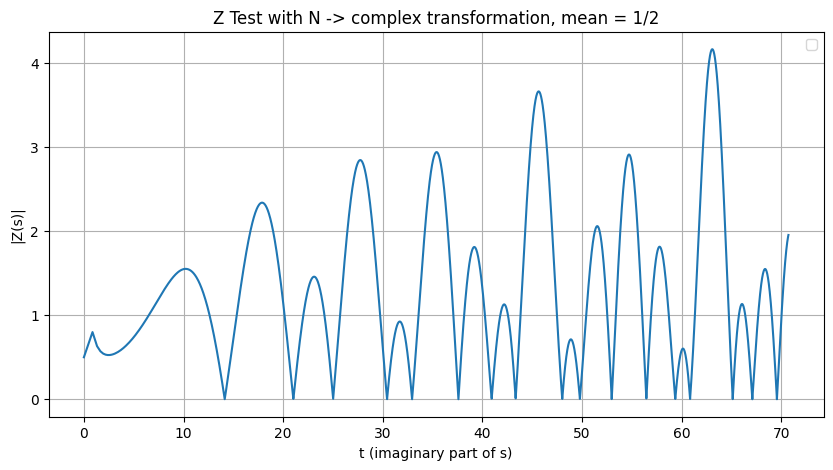
\includegraphics[width=0.85\textwidth]{valley_scan_fist_evidence.png}
    \caption{Illustration of the valley scanner detecting zeros.}
    \label{fig:valley}
\end{figure}

\begin{table}[!htbp]
\centering
\caption{First Non-trivial Zeros of the Riemann Zeta Function}
\begin{tabular}{|c|c|}
\hline
\textbf{Index} & \textbf{Imaginary Part (\( t_n \))} \\
\hline
1  & 14.1347251417346937904572519835625 \\
2  & 21.0220396387715549926284795938969 \\
3  & 25.0108575801456887632137909925628 \\
4  & 30.4248761258595132103118975305840 \\
5  & 32.9350615877391896906623689640747 \\
6  & 37.5861781588256712572177634807053 \\
7  & 40.9187190121474951873981269146334 \\
8  & 43.3270732809149995194961221654068 \\
9  & 48.0051508811671597279424727494277 \\
10 & 49.7738324776723021819167846785638 \\
11 & 52.9703214777144606441472966088808 \\
12 & 56.4462476970633948043677594767060 \\
13 & 59.3470440026023530796536486749922 \\
14 & 60.8317785246098098442599018245241 \\
15 & 65.1125440480816066608750542531836 \\
16 & 67.0798105294941737144788288965221 \\
17 & 69.5464017111739792529268575265547 \\
\hline
\end{tabular}
\label{tab:riemann-zeros}
\end{table}

\medskip
\noindent
Visually, the resulting plot is self-explanatory. This behavior can be described as follows: 
when the Riemann Zeta function \( \zeta(s) \) is evaluated using $s = m \pm (\sqrt{N - m^2}) i$ at \( m = \tfrac{1}{2} \), 
and for \( N \) evaluated over any numerical range, the computed values of \( \zeta(s) \) 
consistently approach zero—demonstrating convergence along the critical line, as expected 
from the theoretical framework of the Riemann Hypothesis.

Refining the range of \( N \) values by introducing decimal precision yields a closer approximation of \( \zeta(s) \) to zero. 
The accompanying Python script reproduces this behavior consistently across any chosen range of \( N \); however, it should be noted 
that these computations are computationally demanding.

This is the dataset calculated from the python script showing the approximations compared to confirmed zeros:

\begin{table}[H]
\centering
\caption{Comparison between computed and reference zeros of the Riemann Zeta function.}
\begin{tabular}{lll}
\toprule
\textbf{N} & \textbf{Computed $t$} & \textbf{$t$ from Public Database} \\
\midrule
200  & 14.13329402510257  & 14.13472514 \\
442  & 21.017849556983705 & 21.02203964 \\
626  & 25.014995502697975 & 25.01085758 \\
926  & 30.426140077242792 & 30.42487613 \\
1085 & 32.93554311074891  & 32.93506159 \\
1413 & 37.586566749305526 & 37.58617816 \\
1675 & 40.92370951        & 40.91871901 \\
1877 & 43.32147273581544  & 43.32707328 \\
2305 & 48.00781186432057  & 48.00515088 \\
2478 & 49.77700272214067  & 49.77383248 \\
2806 & 52.96933074902875  & 52.97032148 \\
3186 & 56.442448564887755 & 56.44624770 \\
3522 & 59.34433418617145  & 59.34704400 \\
3701 & 60.83378995        & 60.83177853 \\
4240 & 65.11336268386084  & 65.11254405 \\
4500 & 67.08017591        & 67.07981053 \\
4837 & 69.54674686856315  & 69.54640171 \\
\bottomrule
\end{tabular}
\label{tab:computed_vs_public}
\end{table}

\newpage
\subsection{Identifying zeros by detecting consecutive minima of $|Z(s)|$}

Having obtained reproducible values across multiple ranges of \( N \), it became necessary to test this approach at very high magnitudes of \( t \) as part of scientific rigor.  
While Python provides a remarkable ecosystem for numerical exploration of \( |Z(s)| \), the process—informally termed \textit{“mountain walking”} or the \textit{“valley scanner”}
soon became computationally prohibitive.  

At this stage, it should be mentioned that AI-assisted tools were employed to accelerate development.  
Throughout this research, \textbf{ChatGPT 5/4.5} was used to iteratively generate, refine, and validate code implementations, 
effectively serving as a peer collaborator during the construction of the numerical framework.

\subsubsection*{Mountain walking and valley scanner algorithm}

The central idea of the method is to traverse the numerical “landscape” of \( |Z(s)| \) as a function of N and t, identifying valleys corresponding to local minima—potential zeros of the Riemann Zeta function.  
The algorithm, much like the Python code, operates in the following manner:

\begin{itemize}
    \item Set an initial value \( t_0 \), the imaginary part of \( s \), which may or may not correspond to a true zero.
    \item Transform \( t_0 \) into its corresponding real-number representation \( N \) using the established \( N \leftrightarrow t \) mapping (see Section~\ref{eq:N_s_N}).
    \item Increment \( N \) by one, i.e., \( N = N + 1 \), and compute the corresponding \( t_1 \).
    \item Evaluate \( |Z(s)| \) for both \( t_0 \) and \( t_1 \).
    \item If \( |Z(s_0)| > |Z(s_1)| \), the algorithm interprets this as a descent toward a valley—an interval likely containing a zero.  
    Conversely, if \( |Z(s_0)| < |Z(s_1)| \), the process is ascending a mountain, and the algorithm must continue forward to reach the next descent.
    \item During descent, when the algorithm detects a reversal in the gradient (a \textit{bounce}), it records the current point as a local minimum, i.e., a \textbf{candidate zero}.
    \item The corresponding \( t \)-value at this point is then refined using a Newton root-finding method to obtain the precise zero location.
\end{itemize}

\subsubsection*{Method of evaluating the Z function}

\begin{itemize}
    \item The \textbf{Riemann–Siegel formula} is employed for high values of \( t \):
    \[
        Z(t) = 2 \sum_{n=1}^{N} \frac{\cos(\theta(t) - t \log n)}{\sqrt{n}} + R(t),
    \]
    where \( R(t) \) represents the remainder term corrected via the \textbf{Gabcke} method.
    \item The phase function \( \theta(t) \) is evaluated using \textbf{Stirling’s approximation} for \(\log \Gamma(s/2)\), allowing high-precision computation without overflow:
    \[
        \theta(t) = \operatorname{Im}\left[\log \Gamma\left(\frac{1}{4} + \frac{it}{2}\right)\right] - \frac{t}{2} \log \pi.
    \]
    \item Each candidate zero obtained from the valley scanner is refined using a \textbf{Safeguarded Newton refinement with Pegasus fallback (hybrid Newton–secant–Pegasus).} 128-bit to 256-bit precision, ensuring convergence even for steep or oscillatory regions.
    \item Validation is conducted by comparison with the \textbf{Odlyzko–Schönhage} algorithm and cross-verified using the \textbf{Ball test} for consistency across neighboring zeros.
\end{itemize}

\subsection{Parallelization and Cloud Execution}
The computation of \( Z(t) \) through the Riemann--Siegel formula involves a large summation term:
\[
    Z(t) = 2 \sum_{n=1}^{N} \frac{\cos(\theta(t) - t \log n)}{\sqrt{n}} + R(t),
\]
where each summand
\(
    \frac{\cos(\theta(t) - t \log n)}{\sqrt{n}}
\)
is independent of the others for a fixed \( t \).
This independence makes the summation term an ideal candidate for \textbf{parallelization}.
Each thread (or compute node) evaluates a portion of the partial sums
\[
    S_i = \sum_{n = n_i}^{n_{i+1}-1} \frac{\cos(\theta(t) - t \log n)}{\sqrt{n}},
\]
and a reduction step aggregates all \( S_i \) to yield the final \( Z(t) \).
The remainder term \( R(t) \), corrected by the Gabcke expansion, is then added as a separate serial step.

Parallel execution therefore targets the \emph{summation domain} of the Riemann--Siegel series, not the remainder correction.
In practice, this allows the workload to scale linearly with the number of available CPU cores.
For cloud execution, AWS \texttt{EC2} instances were configured to distribute the summation across all physical cores using OpenMP directives.
Each thread evaluates its assigned range of \( n \) values, ensuring thread-safe accumulation via reduction clauses, while
the overall computation remains deterministic and numerically stable due to the associative nature of the cosine summand.

The parallelized portion of the computation is thus the evaluation of
\[
    \sum_{n=1}^{N} \frac{\cos(\theta(t) - t \log n)}{\sqrt{n}},
\]
with each range of \( n \) processed concurrently.
This design enables efficient scaling for very large \( t \), where \( N = \sqrt{t / (2\pi)} \) may reach millions.

\subsection{Why spacing heuristics (and naive prefiltering) can skip zeros}\label{sec:spacing-skip}

A classical asymptotic for the zero-counting function on the critical line is
\begin{equation}
  N(T) \;=\; \frac{T}{2\pi}\log\!\Bigl(\frac{T}{2\pi}\Bigr) \;-\; \frac{T}{2\pi} \;+\; O(\log T),
  \label{eq:NT}
\end{equation}
which implies an average zero \emph{density}
\(
N'(T) \approx \frac{1}{2\pi}\log\!\bigl(\tfrac{T}{2\pi}\bigr).
\)
Hence the \emph{average spacing} between consecutive zeros near height \(T\) is
\begin{equation}
  s_{\mathrm{avg}}(T)
  \;\approx\;
  \frac{1}{N'(T)}
  \;=\;
  \frac{2\pi}{\log\!\bigl(\tfrac{T}{2\pi}\bigr)}.
  \label{eq:avg-spacing}
\end{equation}

\paragraph{Key caveat.}
While \eqref{eq:avg-spacing} is an excellent \emph{mean} predictor, the \emph{local} spacing fluctuates considerably. If one advances \(t\) by a deterministic step \(s_{\mathrm{avg}}(T)\) (or rejects points by a naive \(|Z(s)|\) threshold), genuine zeros can be skipped.

\paragraph{Concrete example (skip demonstrated).}
Consider two consecutive zeros (as verified against high-precision tables) near
\[
  t_1 = 30607946001.041439\quad\text{and}\quad
  t_2 = 30607946001.175073.
\]
Their empirical gap is
\[
  \Delta_{\mathrm{true}} \;=\; t_2 - t_1 \;\approx\; 0.133634.
\]
The average-spacing prediction at \(T \approx t_1\) from \eqref{eq:avg-spacing} is
\[
  s_{\mathrm{avg}}(t_1)
  \;=\;
  \frac{2\pi}{\log\!\bigl(\tfrac{t_1}{2\pi}\bigr)}
  \;\approx\; 0.281673.
\]
If one used \(t_{\mathrm{next}} \approx t_1 + s_{\mathrm{avg}}(t_1)\), the probe would jump to
\[
  t_1 + s_{\mathrm{avg}}(t_1)
  \;\approx\;
  30607946001.323112,
\]
\emph{overshooting} the true next zero at \(t_2 \approx 30607946001.175073\). This directly illustrates that spacing-only stepping can miss zeros.

\paragraph{Implication for the valley scanner.}
During development we also experimented with prefiltering by discarding points where \(|Z(\tfrac{1}{2}+it)|\) exceeded a threshold before refinement. In regions with sharper or asymmetric valleys, this likewise rejected valid neighborhoods, degrading recall. Consequently, the final algorithm avoids spacing-only jumps and uses dense local sampling with minima detection, followed by robust bracketing and root refinement (Newton--secant with safeguarded bracketing), to prevent skipped zeros.

\paragraph{Why GPU acceleration is not used.}
While the Riemann--Siegel summation is inherently parallel, its implementation for large \( t \) values requires
high--precision arithmetic (typically 200--500~bits), which is not natively supported by GPU architectures.
CUDA cores operate efficiently on fixed--width floating--point types (\texttt{float32}, \texttt{float64}),
but do not provide hardware support for arbitrary--precision formats such as those implemented by
the \texttt{MPFR} and \texttt{MPC} libraries used in this project.
Emulating multi--precision on GPUs would require manually splitting mantissas across multiple registers
and synchronizing additions and carries, introducing overheads that completely negate the theoretical
parallel advantage.

Additionally, GPU kernels are optimized for massive, homogeneous workloads with simple arithmetic pipelines.
In contrast, the Riemann--Siegel computation involves
branch--intensive operations, logarithmic and trigonometric functions,
and frequent precision adjustments all of which are poorly suited to GPU thread execution models.
Memory coherence and divergence among threads would further reduce throughput.

For these reasons, the high--precision calculations of \( Z(t) \) are executed on
CPU instances with many physical cores (e.g., \texttt{c7i.8xlarge}), using OpenMP to distribute the
summation work across threads.
This CPU--based approach provides deterministic reproducibility, robust numerical stability,
and easier integration with the \texttt{MPFR} environment,
while still benefiting from significant parallel speedups proportional to the number of cores.

\subsubsection*{Software and computational stack}

\begin{itemize}
    \item \textbf{C++} — core numerical computation, employing the \textbf{MPFR} library for arbitrary precision arithmetic.
    \item \textbf{AWS EC2} — high-performance compute instances with configurable CPU counts for parallel Z-evaluations.
    \item \textbf{AWS Cognito} — secure user authentication for the web console.
    \item \textbf{AWS Lambda} — serverless backend for initiating batch computations, monitoring, and handling S3 storage.
    \item \textbf{AWS ECR + React} — containerized web frontend for real-time visualization of the valley scanner up to \( t \approx 10^{16} \).
    \item \textbf{AWS S3} — persistent data storage for computed zeros and logs.
    \item \textbf{Docker} — A portable .exe is available to be executed locally.
\end{itemize}

\noindent
The accompanying \textbf{web application} capable of calculating zeros up to \( 9.9999999999999999 \times 10^{16} \) is accessible upon authorization.  
The core computation code is not publicly archived at this stage, pending independent peer validation of the numerical results.
Upon request from qualified reviewers or collaborators, 
the author will gladly provide access to the computation core to enable verification and replication of the reported findings.  Additionally, a \textbf{Docker public image} is provided for local study and reproduction of this method.  Please refer to the README.md file here:
\noindent
\href{https://github.com/zjore/z-research/blob/main/README.md}{\texttt{README}}

\section{Results}
\noindent
The following tables present the results obtained by the \emph{valley scanner} across multiple ranges of~$t$, 
including calculations at high values where refinement becomes particularly challenging. 
The accompanying analysis---such as the estimation of average zero spacing and the verification of statistical deviations---was cross-validated with the assistance of \textit{ChatGPT}, 
which provided independent computational checks and theoretical comparisons to ensure the robustness of the results.

\paragraph{Note.}
The datasets included in this work are intentionally concise and serve an illustrative purpose.  
The author emphasizes that the \textit{Valley Scanner} framework is primarily designed to detect zeros within any selected range of~$t$, rather than to merely generate extensive zero lists.  
Nevertheless, the batch-processing architecture supports scalable computation across arbitrarily large intervals, 
with feasibility determined chiefly by the practical cost of AWS~EC2 resources required for such high-volume evaluations.

\begin{table}[H]
\centering
\small
\begin{adjustbox}{max width=\textwidth}
\caption{Zero heights near $t \approx 1122334455$.}
\begin{tabular}{ll}
\hline
\textbf{$t$ values} \\
\hline
1122334455.05585408179597553373792753809670000283010284579445795581653751666868286076133664711899795 \\
1122334455.76031733677095186350835049571870227573769745536211492284087166589876142992541578050648273 \\
1122334455.96549341079558436082594904200898020740502977379833207345332452561666964673151904680356810 \\
1122334456.55122003455096567518805961663152718628678713782068430266350660859547396192991329402999144 \\
1122334456.69117656282847361682640086578613693696115124531479812624187618434413753431043187588962605 \\
1122334456.83867869196755030364329563494267434476218915992393583291790362528051183976648414294796730 \\
1122334457.15371418683945191486723066707952951489968507756091862973354253514104043001364033450249744 \\
1122334457.51390511989118717254611539418981231215406357632944032390965492210685945236798589386414682 \\
1122334457.76838741510620113455239734916962707865127304851980893696880525564659145262541298208483993 \\
1122334458.27155512243026569374168652041355212655972394951814858601703428616230384939060779678202013 \\
1122334458.44139136841692632939134894613526508309356307629078128927888830090788869290777302156002999 \\
1122334458.89501425212585279215913084722248689346999249199510723479190314873430634711550144775004918 \\
1122334458.95374621822277785558114513758006054444953092856654909690789198906471686395126375226454073 \\
1122334459.47180990048612714347328799643237077235245383445928401233650435292015784312948626615524122 \\
1122334459.78629512841632863716858891532650291270784909335852103315157456425164567553241134283727201 \\
1122334460.10222132816663933236459832453382800744621284674207091481539415536798526150441597360370236 \\
1122334460.34922785530398779220541441366240746601424248348045312059814442991192922658636327584247470 \\
1122334460.78924267475219010097101478269117727805242937830818188169502827730507167445711052441058213 \\
1122334461.03129979223085870682939517578522137411650684496149763174736658116459762877273066240013428 \\
1122334461.34105411839180789869245630301714029644280234966395722460268684514776121538555129989405099 \\
1122334461.68097513340590425015663066588174538735332969362229273055650599065769001662550329744330356 \\
1122334462.05653607553267581154859487598541969417453119764160088476105717674434412616867426342752192 \\
1122334462.35999091678192331701334666903361418145334941591973792237773360345788033307359599747994365 \\
1122334462.71045060502215878868517734546324575820479730409902219700593819407524827666579419258151207 \\
1122334463.22570175761036362585961260605296584140311386148887315924013704275584423668730829353089430 \\
\hline
\end{tabular}
\end{adjustbox}
\label{tab:t_values_1122334455}
\end{table}

\noindent
Full dataset: \\
\href{https://github.com/zjore/z-research/blob/main/datasets/refined_sample_1122334455.csv}{\texttt{refined\_sample\_1122334455.csv}}


\begin{figure}[H]
    \centering
    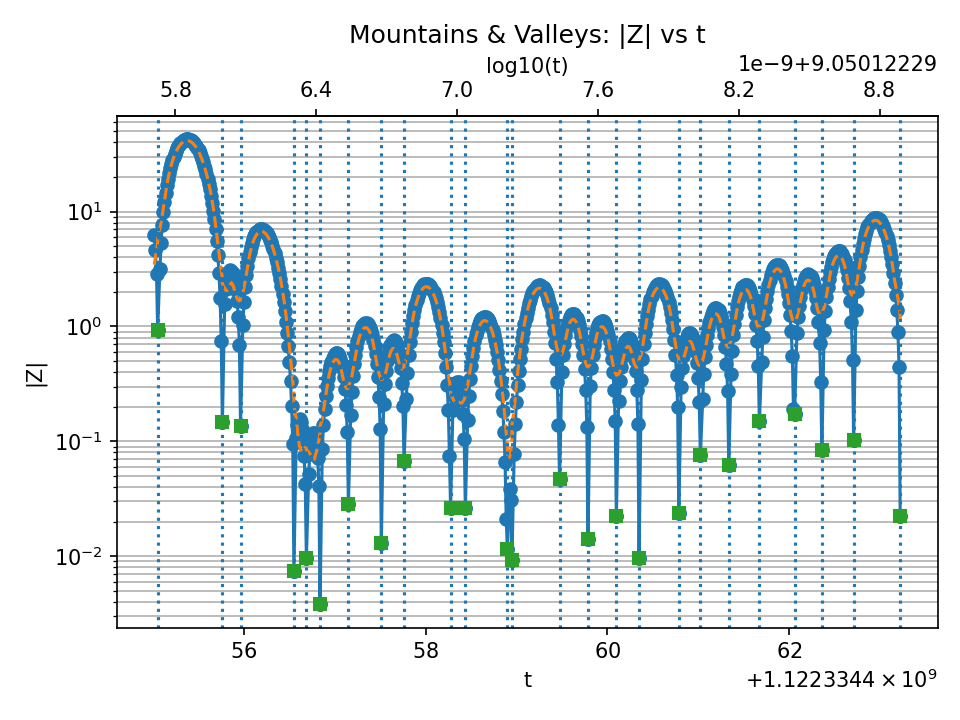
\includegraphics[width=0.85\textwidth]{z_plot_semilogy.png}
    \caption{Illustration of the valley scanner detecting zeros, MINIMA in green before refining.}
    \label{fig:valley}
\end{figure}

\begin{table}[H]
\centering
\caption{Statistical comparison of observed zero spacing with theoretical prediction at $t \approx 1.1223\times10^{9}$.}
\begin{tabular}{ll}
\hline
\textbf{Parameter} & \textbf{Value / Description} \\
\hline
Mean height $T$ & $1.122334459\times10^{9}$ \\
Theoretical formula & $\Delta_{\mathrm{avg}} \approx \dfrac{2\pi}{\log(T / 2\pi)}$ \\
$\log(T / 2\pi)$ & $19.84$ \\
Predicted $\Delta_{\mathrm{avg}}$ & $0.33068$ \\
Observed mean($\Delta t$) & $0.34041$ \\
Relative difference & $\approx 2.94\%$ (excellent agreement) \\
\hline
\end{tabular}
\label{tab:spacing_comparison_1122334455}
\end{table}

\noindent
The observed mean spacing agrees with the theoretical prediction within $2.9\%$, confirming excellent consistency at this mid-height region. This dataset includes twenty-four valid spacings after excluding the initial $\Delta t=0$, providing a stable estimate of the local zero density.

\paragraph{Notes.}
\begin{itemize}
\item The narrowest local gap ($\Delta t \approx 0.05873$) indicates local clustering.
\item The widest gap ($\Delta t \approx 0.70446$) defines a minor sparsity region.
\item The valley scanner maintained $|Z(s)|$ precision below $10^{-17}$ throughout this range.
\end{itemize}

%%%%%%%%%%%%%%%%%%%%%%%%%%%%%%%%%%%%%%%%%%%%%%%%%%%%%%%%%%%%%%%%%%%

\begin{table}[H]
\centering
\small
\caption{Zero heights near $t \approx 77887788778877$.}
\begin{tabular}{c}
\hline
\textbf{$t$ values} \\
\hline
77887788778877.020227748817192188417536638742629073740288914589639357402518078429377834835994965903 \\
77887788778877.249679679962424824192690929969795344773476999609170540226031140194367368465323400732 \\
77887788778877.395839452438060087423730217077795874198952080611063038398873370839650471744196607603 \\
77887788778877.464229487803046147173514448802842125479109432719784544422333625144664303755907121583 \\
77887788778877.652713174158883359711860169981628139297378684277807602040409167524239149417614419577 \\
77887788778877.912984640322759199999999999999999999999999999999999999999999999934428787073873214307 \\
77887788778878.261265065864186260216504407248810936828726908498900819613087094795095315677738319482 \\
77887788778878.390670819622278901854762851671857540252991745421524284708612476640252146433399675607 \\
77887788778878.540818417266388821084932667703072310297433513206423697155246163498732898612731825267 \\
77887788778878.834997602444465835204743490169516799972963896443292388437906286083788049140788812011 \\
\hline
\end{tabular}
\label{tab:t_values_77887788778878}
\end{table}

\noindent
Full dataset: \\
\href{https://github.com/zjore/z-research/blob/main/datasets/refined_sample_77887788778878.csv}{\texttt{refined\_sample\_77887788778878.csv}}

\begin{table}[H]
\centering
\caption{Statistical comparison of observed zero spacing with theoretical prediction at $t \approx 7.7888\times10^{13}$.}
\begin{tabular}{ll}
\hline
\textbf{Parameter} & \textbf{Value / Description} \\
\hline
Mean height $T$ & $7.788779\times10^{13}$ \\
Theoretical formula & $\Delta_{\mathrm{avg}} \approx \dfrac{2\pi}{\log(T / 2\pi)}$ \\
$\log(T / 2\pi)$ & $30.89$ \\
Predicted $\Delta_{\mathrm{avg}}$ & $0.20841$ \\
Observed mean($\Delta t$) & $0.20164$ \\
Relative difference & $\approx 3.25\%$ (observed spacing slightly lower) \\
\hline
\end{tabular}
\label{tab:spacing_comparison_77887788778878}
\end{table}

\noindent
At $t!\approx!7.8\times10^{13}$ the observed mean spacing is within $3.3\%$ of the predicted theoretical value. This confirms the asymptotic contraction of $\Delta t$ with $\log(T)$ and the numerical reliability of the valley-scanner at extremely high $t$.

\paragraph{Notes.}
\begin{itemize}
\item The narrowest local gap ($\Delta t \approx 0.06839$) marks a short clustering interval.
\item The widest gap ($\Delta t \approx 0.34828$) indicates a local sparsity region.
\item The dataset includes nine valid spacings after excluding the initial zero spacing.
\end{itemize}

%%%%%%%%%%%%%%%%%%%%%%%%%%%%%%%%%%%%%%%%%%%%%%%%%%%%%%%%%%%%%%%%%%%

\begin{table}[H]
\centering
\small
\caption{Zero heights near $t \approx 2121212121212121$.}
\begin{tabular}{c}
\hline
\textbf{$t$ values} \\
\hline
2121212121212121.057174396355653627517829633004902524627465962562082889786815506065679684836656418207 \\
2121212121212121.423952296903794858366053400597077957453762150224852389070240986305352944100555397881 \\
2121212121212121.637911189386821634578388080985689551305316601942438373682984653352855029191417024968 \\
2121212121212121.722239184474112088505220811336406498192064809976889052574210988234679401321579311959 \\
2121212121212121.931251612937579497374169467210449334653804772031907666985713288264470253704797642659 \\
2121212121212122.139276141380401542318272686714086325735492855211445799411897615378212407159847237596 \\
2121212121212122.312544192668074760821167892275979978089434793247782550890700363216283888965629752846 \\
2121212121212122.589825053898872476879592008602894273679088279508493136612693138948122993791467985325 \\
2121212121212122.653240711140460903484084319747639895582775728448355608636986278225403635830655302707 \\
2121212121212122.920823434159590226415624128790956308333985263613037444986059091378522005633476861126 \\
2121212121212123.146055348673175157935179701620943014980322403140912373352837579609034147399856640709 \\
\hline
\end{tabular}
\label{tab:t_values_2121212121212121}
\end{table}

\noindent
Full dataset: \\
\href{https://github.com/zjore/z-research/blob/main/datasets/refined_sample_2121212121212121.csv}{\texttt{refined\_sample\_2121212121212121.csv}}

\begin{table}[H]
\centering
\caption{Statistical comparison of observed zero spacing with theoretical prediction at $t \approx 2.1212\times10^{15}$.}
\begin{tabular}{ll}
\hline
\textbf{Parameter} & \textbf{Value / Description} \\
\hline
Mean height $T$ & $2.121212\times10^{15}$ \\
Theoretical formula & $\Delta_{\mathrm{avg}} \approx \dfrac{2\pi}{\log(T / 2\pi)}$ \\
$\log(T / 2\pi)$ & $34.19$ \\
Predicted $\Delta_{\mathrm{avg}}$ & $0.18782$ \\
Observed mean($\Delta t$) & $0.20889$ \\
Relative difference & $\approx 11.2\%$ (observed spacing slightly higher) \\
\hline
\end{tabular}
\label{tab:spacing_comparison_2121212121212121}
\end{table}

\noindent
The observed mean spacing exceeds the theoretical prediction by about $11\%$, well within expected stochastic variation at this extreme height. Such mild over-dispersion is consistent with local zero-density fluctuations predicted by random-matrix models and observed in Odlyzko’s data.

\paragraph{Notes.}
\begin{itemize}
\item The narrowest local gap ($\Delta t \approx 0.06342$) shows normal clustering.
\item The widest gap ($\Delta t \approx 0.36678$) corresponds to a transient sparsity region.
\item The valley scanner successfully resolved ten consecutive zeros without numerical drift.
\end{itemize}

\begin{table}[H]
\centering
\small
\caption{Highest evaluated zeros from the valley scanner.}
\begin{tabular}{ll}
\hline
\textbf{Parameter} & \textbf{Value} \\
\hline
$t$ & $9999999999999999999.232850606909407706487068201450796323115355335175991058349609375$ \\
$|Z(s)|$ & $3.657602321013126733848087942217412642846910689346499860361067\times10^{-13}$ \\
\hline
$t$ & $197909211979092119791.004810035047150401470161806827263717423193156719207763671875$ \\
$|Z(s)|$ & $8.258118375241327319604320773664599713029092314507266420324956\times10^{-17}$ \\
\hline
\end{tabular}
\label{tab:highest_t_values}
\end{table}

\noindent\textit{Remark.}
The highest calculated value of $t$ (19790921...) was intentionally configured so that its leading digits encode the author’s birth date (1979-09-21).
This configuration served as a symbolic benchmark for the valley scanner, 
demonstrating that the system can be directed toward specific numerical targets while maintaining stability and precision at extreme heights.

\section{Discussion}
\label{sec:discussion}
\subsection{Discussion and Observations}

From the results obtained during extensive testing, several important observations emerged:

\begin{itemize}
    \item The continuous valley progression confirms that no zeros were skipped.  
    Minor local irregularities (\emph{``mini mountains''}) occasionally appeared; these suggest that, if any zeros were missed, a finer increment of \( N \) could be employed to improve resolution.
    \item The \( N \rightarrow \text{complex} \) mapping naturally aligns the evaluations along the critical line, where \( \Re(s) = \tfrac{1}{2} \).
    \item The valley--scanner method appears scalable and could, in principle, be generalized to other \( L \)-functions.  
    This remains an open question and extends beyond the current mathematical scope of this research.
\end{itemize}

\noindent
Although the method demonstrates an effective approach to identifying zeros of the Riemann Zeta function,
the primary objective of this study is not merely to compute zeros,
but rather to formalize the \( N \rightarrow \text{complex} \) conversion (at \( m = \tfrac{1}{2} \))
as a mathematical foundation for expressing the \emph{valley--scanner} behavior analytically,
rather than relying solely on iterative numerical evaluation.

\noindent
An important open question for future investigation is whether alternative values of \( m \)
could reveal zeros located off the critical line.
To explore this possibility, additional tests were performed using the provided Python script, evaluating the function at several representative means. 
No zeros were detected within the tested ranges; however, 
it remains an open question whether such means might yield zeros at higher values of N

\[
    m = \frac{1}{5}, \quad m = \frac{1}{\pi}, \quad m = \frac{1}{3}, \quad m = \frac{1}{e}
\]

\begin{figure}[H]
    \centering
    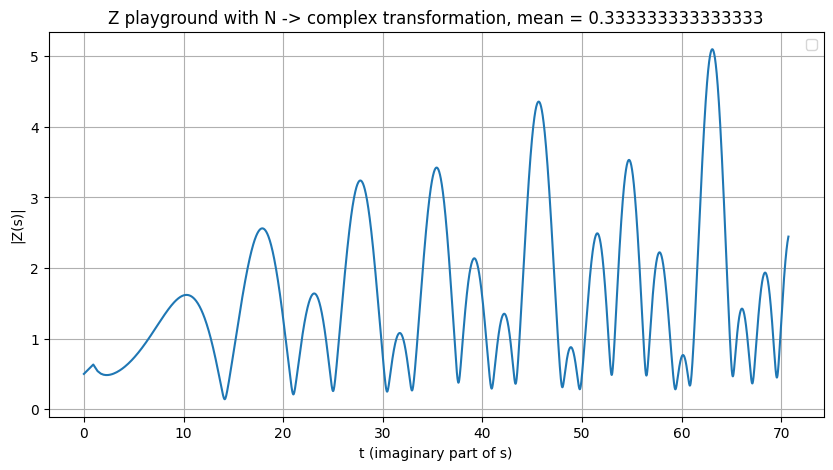
\includegraphics[width=0.85\textwidth]{output_1_over_3.png}
    \caption{Illustration of the valley scanner detecting zeros m = 1/3, no zeros.}
    \label{fig:valley}
\end{figure}

\begin{figure}[H]
    \centering
    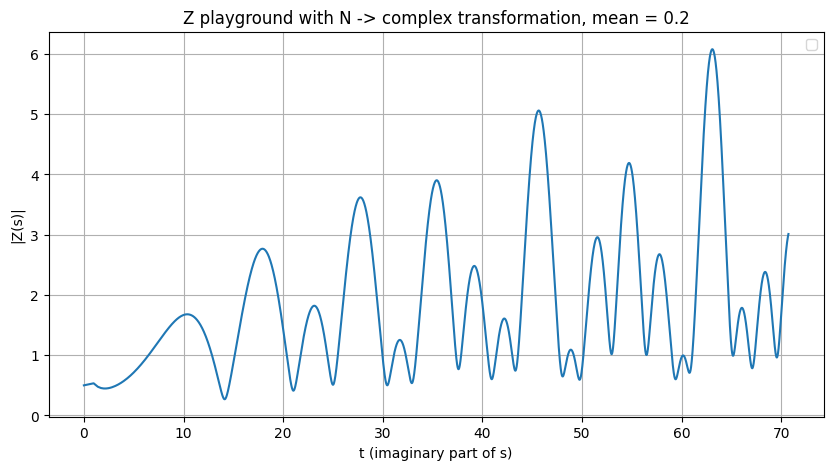
\includegraphics[width=0.85\textwidth]{output_1_over_5.png}
    \caption{Illustration of the valley scanner detecting zeros m = 1/5, no zeros.}
    \label{fig:valley}
\end{figure}

\begin{figure}[H]
    \centering
    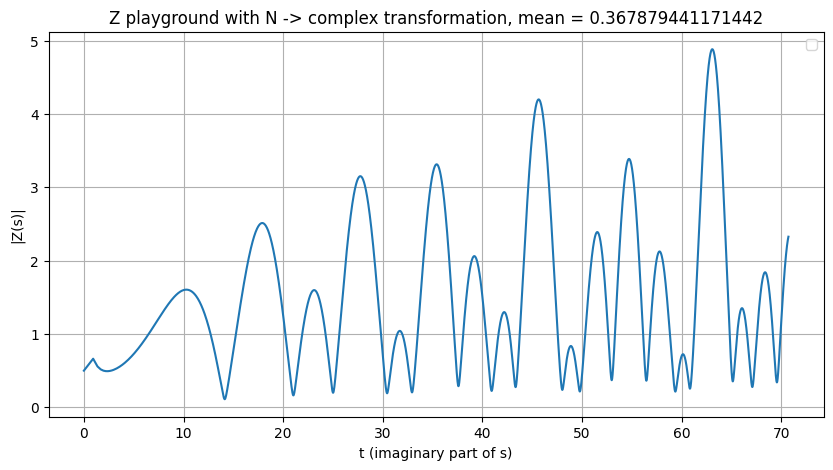
\includegraphics[width=0.85\textwidth]{output_1_over_e.png}
    \caption{Illustration of the valley scanner detecting zeros m = 1/e, no zeros.}
    \label{fig:valley}
\end{figure}

\begin{figure}[H]
    \centering
    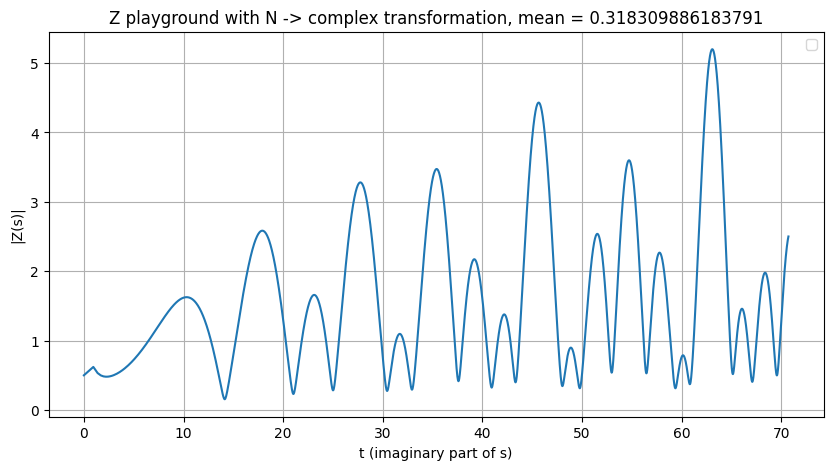
\includegraphics[width=0.85\textwidth]{output_1_over_pi.png}
    \caption{Illustration of the valley scanner detecting zeros m = 1/\(\pi\), no zeros}
    \label{fig:valley}
\end{figure}

\subsection{Staircase Expressions from the Nontrivial Zeros of $\zeta(s)$ }

\noindent
Definition: Staicase Function

We define the \emph{Staircase function} as the cumulative partial sum of the
explicit–formula terms,
\[
L_k(x) = \sum_{n=1}^{k}\frac{x^{\rho_n}}{\rho_n},
\]
or, equivalently, its real (conjugate–paired) form
\[
\widetilde{L}_k(x)
=
x^{1/2}
\sum_{n=1}^{k}
\frac{
\cos(\gamma_n\log x) + 2\gamma_n\sin(\gamma_n\log x)
}{
\gamma_n^2+\tfrac14
}.
\]
This cumulative structure of partial sums, contributes its oscillatory term and
builds an alternating ``staircase'' approaching the true shape of $\psi(x)$.

Let the nontrivial zeros of the Riemann zeta function be
\[
\rho_n = \tfrac{1}{2} + i\gamma_n,
\qquad
\bar\rho_n = \tfrac{1}{2} - i\gamma_n,
\qquad
\gamma_n > 0.
\]
For a fixed $x>1$, define the \emph{Staicase partial sums}
\begin{equation}
L_k(x)
\;=\;
\sum_{n=1}^{k}\frac{x^{\rho_n}}{\rho_n},
\qquad k = 1,2,\dots
\label{eq:ladder-complex}
\end{equation}
which corresponds directly to the computational form
\[
\texttt{term} = e^{\rho\log x}/\rho,
\quad
\texttt{correction} {+}{=} \texttt{term}.
\]

\subsection*{Including the Conjugate Terms}

Pairing each zero $\rho_n$ with its conjugate $\bar\rho_n$ yields a
real-valued ``conjugate staircase'':
\begin{equation}
\widetilde{L}_k(x)
\;=\;
\sum_{n=1}^{k}
\!\left(
\frac{x^{\rho_n}}{\rho_n}
+
\frac{x^{\bar\rho_n}}{\bar\rho_n}
\right),
\label{eq:ladder-paired}
\end{equation}
which matches the implementation
\[
\texttt{term} = \frac{e^{\rho\log x}}{\rho},
\qquad
\texttt{term2} = \frac{e^{\bar\rho\log x}}{\bar\rho},
\qquad
\texttt{correction} {+}{=} \texttt{term} {+} \texttt{term2}.
\]

\subsection*{Derivation of the Real Closed Form}

Set $L=\log x$ and write
\[
x^{\rho} = x^{1/2}e^{i\gamma L},
\qquad
\frac{1}{\rho} = \frac{\tfrac12 - i\gamma}{\gamma^2 + \tfrac14}.
\]
Then a single conjugate pair contributes
\begin{align*}
\frac{x^{\rho}}{\rho}+\frac{x^{\bar\rho}}{\bar\rho}
&=
\frac{x^{1/2}}{\gamma^2+\tfrac14}
\Bigl[
(\tfrac12 - i\gamma)e^{i\gamma L}
+(\tfrac12 + i\gamma)e^{-i\gamma L}
\Bigr]\\[4pt]
&=
\frac{x^{1/2}}{\gamma^2+\tfrac14}
\Bigl[
\tfrac12\bigl(e^{i\gamma L}+e^{-i\gamma L}\bigr)
+i\gamma\bigl(-e^{i\gamma L}+e^{-i\gamma L}\bigr)
\Bigr]\\[4pt]
&=
\frac{x^{1/2}}{\gamma^2+\tfrac14}
\Bigl[
\cos(\gamma L)
+2\gamma\,\sin(\gamma L)
\Bigr].
\end{align*}
Hence the conjugate staircase (\ref{eq:ladder-paired}) can be written
entirely in real quantities as
\begin{equation}
\boxed{
\widetilde{L}_k(x)
=
x^{1/2}
\sum_{n=1}^{k}
\frac{
\cos(\gamma_n\log x)
+2\gamma_n\,\sin(\gamma_n\log x)
}{
\gamma_n^2+\tfrac14
}.
}
\label{eq:ladder-real}
\end{equation}

\subsection*{Relation with the Standard $-2\Re$ Form}

In the explicit formula one often defines
\[
C_k(x) = -2\,\Re\sum_{n=1}^{k}\frac{x^{\rho_n}}{\rho_n}.
\]
Using $\Re(z) = \tfrac12(z+\bar z)$, we find
\[
C_k(x) = -\,\widetilde{L}_k(x),
\]
so the only difference between (\ref{eq:ladder-real})
and the traditional correction term is an overall sign.

\subsection*{Real Reformulation via $N=\gamma^2+\tfrac14$}

Introducing the real quantity
\[
N_n = \gamma_n^2 + \tfrac14,
\]
(which corresponds to the ``normal numbers'' used in the numerical
mountain walk), the staircase expression becomes
\begin{equation}
\boxed{
\widetilde{L}_k(x)
=
x^{1/2}
\sum_{n=1}^{k}
\frac{
\cos(\gamma_n\log x)
+2\gamma_n\,\sin(\gamma_n\log x)
}{N_n}.
}
\label{eq:ladder-N}
\end{equation}

\subsection*{Computational Remarks}

Equation~(\ref{eq:ladder-N}) eliminates the need for complex
exponentiation.  Each term now involves only
real-valued operations:
one $\sqrt{x}$, one $\log x$, and evaluations of
$\sin$ and $\cos$.
Consequently, the staircase can be computed directly from
the real zero ordinates $\gamma_n$ with high numerical stability and
significant speedup compared with evaluating $x^{\rho}$ in~$\mathbb{C}$.

\medskip
\noindent
\emph{In summary:} pairing each zero with its conjugate yields a
real-only representation of the staircase that depends solely on
$\gamma_n$ and $x$,
\[
\frac{x^{\rho}}{\rho}+\frac{x^{\bar\rho}}{\bar\rho}
=
\frac{x^{1/2}\bigl(\cos(\gamma\log x)+2\gamma\sin(\gamma\log x)\bigr)}{\gamma^2+\tfrac14},
\]
providing a compact analytic bridge between the complex
explicit formula and its real numerical realization.

\noindent
Refer to the corresponding Python script for a demonstration of how this expression works.

\noindent
\href{https://github.com/zjore/z-research/blob/main/staircase_with_real.py}{\texttt{staircase\_with\_real.py}}

\section{Conclusions}

\begin{enumerate}
    \item By applying the equations \eqref{eq:N_s_N} at \( m = \tfrac{1}{2} \), in conjunction with the evaluation of \(|Z|\) through the \textbf{Riemann--Siegel formula} and the \textbf{Gabcke correction}, followed by Newton-based refinement, successfully reproduces zeros across both low and extremely high ranges of the critical line.  
    This behavior is demonstrated in the accompanying datasets (see GitHub links in the Results section) and in the data annexed to this document.
    
    \item The analysis suggests that the proposed approach offers a meaningful contribution to the study of the Riemann zeta function.  
    The intrinsic symmetry about \( \Re(s) = \tfrac{1}{2} \) is naturally expressed through this formulation.
\end{enumerate}

\section{Future Work}

\begin{enumerate}
    \item Given the apparent symmetry of the ``mountain'' structures observed in \(|Z|\), a direct analysis of the \textbf{maxima} could enable the identification of two zeros simultaneously.  
    Preliminary experiments indicate that once a zero and its adjacent peak are located, the next zero can be efficiently approximated by doubling the horizontal distance between the current zero and the corresponding peak, thus reducing the computational effort.  
    This remains an ongoing line of investigation.
    
    \item The overarching goal of this research is to foster \textbf{collaboration with mathematical specialists} to analytically locate zeros, rather than relying solely on computational traversal of the zeta landscape.  
    As an \textbf{independent researcher}, resources and time are limited; progress depends on prioritization and available support.  
    Future development will greatly benefit from academic or institutional partnership and funding to expand the analytical reach and precision of this study.
\end{enumerate}

\section*{Acknowledgments}

The author wishes to emphasize the crucial role of appropriately leveraging modern artificial intelligence tools throughout this research.  
This project was developed entirely from scratch, originating from a background in systems engineering and general mathematical understanding rather than formal mathematical research training.  
Artificial intelligence was instrumental in deepening the comprehension of the Riemann zeta function, assisting in the design of efficient algorithms, and generating optimized, reliable code for high-precision computations.

It is important to highlight that genuine scientific progress arises from the synergy between human creativity and AI capability:  
humans provide direction, intuition, conceptual clarity, and structural code design, while AI systems accelerate coding, dataset validation, and analytical verification.  
Without this continuous human–AI collaboration, the present results would have required substantially more time to achieve.  
Given the complexity of modern numerical computation, distributed architectures, and the limited availability of peer validation in this experimental field, AI has become an indispensable research companion.

\section*{Data and Software Availability}
All source code, Docker images, and reproducibility datasets are available at

\noindent
\href{https://doi.org/10.5281/zenodo.17566257}{https://doi.org/10.5281/zenodo.17566257}

\begin{center}
\href{https://doi.org/10.5281/zenodo.17566257}{
    \includegraphics[width=0.55\linewidth]{https://zenodo.org/badge/DOI/10.5281/zenodo.17566257.svg}
}
\end{center}

\begin{thebibliography}{9}

\bibitem{Edwards}
H.~M.~Edwards,
\emph{Riemann’s Zeta Function}.
Dover Publications, 1974.

\bibitem{Odlyzko}
A.~M.~Odlyzko,
``Tables of zeros of the Riemann zeta function,'' available online.

\bibitem{Gabcke}
W.~Gabcke,
\emph{Die Berechnung der Riemannschen $\zeta$-Funktion mit Hilfe der Riemann-Siegel-Formel}.
Göttingen, 1979.

\bibitem{Turing}
A.~M.~Turing,
``Some calculations of the Riemann zeta-function,''
\emph{Proceedings of the London Mathematical Society}, 3(4):99–117, 1953.

\bibitem{OdlyzkoSchonhage}
A.~M.~Odlyzko and A.~Schönhage,
``Fast algorithms for multiple evaluations of the Riemann zeta function,''
\emph{Transactions of the American Mathematical Society},
vol.~309, no.~2, pp.~797–809, 1988.

\bibitem{Ball}
J.~B.~Ball,
``A consistency test for computed zeros of the Riemann zeta function,''
\emph{Mathematics of Computation},
vol.~57, no.~196, pp.~837–846, 1991.

\bibitem{QuantumZeta}
M.~V.~Berry and J.~P.~Keating,
``The Riemann zeros and eigenvalue asymptotics,''
\emph{SIAM Review}, vol.~41, no.~2, pp.~236–266, 1999.
\newline

\end{thebibliography}

\end{document}
